\chapter{Overview}
This chapter gives an high-level overview of the whole platform, still omitting design and implementation specific details. Firstly, architecture in different deployment modes is described followed by explanation of distributed trace collection. Next, the overview of all pieces of whole platform - the native instrumentation agent and instrumentation server, the user interface used for presenting the observed results and the span savers and data collectors for transporting data from the application node to the user interface server. This chapter ends by a single use case which may help reader to image how this platform can be used in a real-world scenario.
\section{Architecture Description}
The whole platform consist of several pieces. The native agent which is attached to the Java application, the Instrumentation server used for performing the instrumentation in the separated JVM process and the user interface. Data are brought to user interface using various collectors. The platform was designed to be configurable and therefore we support several deploying methods. The instrumentation server can be either on the network available to all the application nodes and can be shared by all applications. This has an advantage of caching the instrumented classes. So when any class is instrumented for the first time, the instrumentation is not performed for other nodes but the class is immediately sent. The disadvantage of this solution is higher latence between the agent and the instrumentation server since they are usually not on the same node. In this case the instrumentation server has to be manually started in advance. Architecture of this scenario is depicted on the diagram \ref{fig:shared_server}.

\begin{figure}
	\centering
	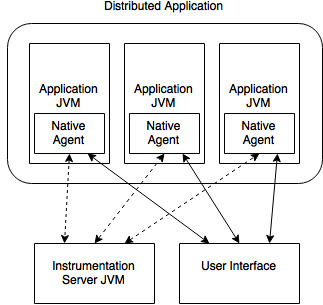
\includegraphics[scale=0.8]{shared_server.png}
	\caption{Architecture with shared instrumentation server. The dotted lines represents the communication between instrumentation server and the agent whilst the regular lines represents data collection from the agent to the UI}
	\label{fig:shared_server}
\end{figure}

The other deployment method is that the instrumentation server runs on each application node. This has the advantage of faster communication since we can use inter-process communication methods to communicate between monitored JVM and the instrumentation server. The disadvantage of this solution is that we have to instrument all classes on each node since there is no communication between the instrumentation servers. In this solution, the server is started automatically during the native agent initialization. Architecture of this scenario is depicted on the diagram \ref{fig:separated_server}.

\begin{figure}
	\centering
	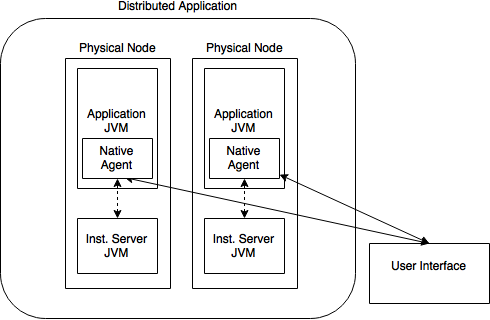
\includegraphics[scale=0.8]{separated_server.png}
	\caption{Architecture with separated instrumentation server. The meaning of the lines is the same as on the diagram above.}
	\label{fig:separated_server}
\end{figure}

\section{Spans}
Spans are the main tool used for capturing distributed traces. They are special classes which instances are injected to instrumented classes to keep track of the communication and the state between the nodes in the distributed application. Usually, the initiator creates so called parent span and new calls started within the span creates new nested spans. The only information required to be available in Span class is its id and parent span id and in order to be able to distinguish different spans, also unique trace id which is created during root span creation. 

Created spans are processes using different span savers and can be send to the user interface using various data collectors.
\section{Span Savers \& Data Collectors}
The platform allows the user to create custom span savers which can be used to plug-in custom data collectors. By default, the platform supports 2 simple span savers:
\begin{itemize}
	\item The default span saver sends asynchronously the collected span to the user interface right away. In this case the functionality of span saver and data collector is covered by this single saver. This span saver should be used for demonstration purposes only since it could overload the user interface or network when there is a high amount of collected spans in a short amount of time.
	\item The second available span saver saves asynchronously the collected data on the disk in the format known to Zipkin UI. This data can be collected using various data collectors. This is a preferred way when putting this tool to production with combination in some well-known data collection agent.
\end{itemize}
\section{User Interface}
The user interface receives the data from the span savers or data collectors and present them to the user. It connects the spans collected from different nodes using the span and parent span ids which means we can see the distributed traces graphically and see how the computation went node by node. For the purpose of this tool, Zipkin User Interface is used for this purpose since it's open source and fulfills exactly the required service. However as mentioned above, the users can write custom span savers to save the data in a format known to different user interface in order to not depend on Zipkin UI.
\section{Native Agent}
The native agent is the core part of the whole platform. It is attached to the monitored application and allows us to obtain various low-level information from the application run. The native agent is responsible for starting the instrumentation server in case of local instrumentation mode or connecting to the instrumentation server when sharing the server between all application nodes.

The main task for the agent is to check weather a class is required to be instrumented and if yes, send the class for the instrumentation to the server and wait for the instrumented code. The agent does not know which classes are to be instrumented and it therefore needs to query the server. The other approach could be to specify which classes should be instrumented as arguments to the client but that would be hard to manage since it would be static list of classes. In this approach the developer can specify which classes can be instrumented on the instrumentation server using simple Byte Buddy API.

The communication protocol between the agent and instrumentation server as well as the technical aspects of the instrumentation are described in the following chapters.
\section{Instrumentation Server}
The instrumentation server is responsible as the name suggest for instrumenting the byte code. The native agent asks the server weather the class is required to be instrumented, the server then received the byte code, performs the instrumentation and sends the data back to the agent. It does not contain any application state and does not know about the distributed traces.

The instrumentation server needs to deal with several technical problems. The main issue is that the classes which are about to be instrumented require all other dependent classes to be available as well. The other issue is for example instrumenting the classes with circular dependencies. The server also performs several optimizations to provide faster response to the agent such as caching the instrumented classes or minimizing the communication when possible. The technical aspects of the issues and the optimizations mentioned above are described in the following sections.
\section{Example Use Case}
In order to have a better understanding how this platform can be used we provide simple use case. Let's assume we 